\documentclass[onecolumn]{article}
\usepackage{graphicx}
\usepackage{float}
\usepackage{hyperref}
\restylefloat{figure}
\begin{document}

\title{Correlation coefficients for sets of random numbers}

\author{Arjen Markus}

\maketitle

\section*{Introduction}
Correlation coefficients are in general useful measures to determine how much of one variable is determined by
another variable. They do not indicate a causal relationship, as should always be stressed. Just think of
a correlation like the number of firemen and the total damage of a fire. Still, they are useful. But
correlation coefficients can be surprisingly large: a wide cloud of data points can still have a correlation
coefficient that is appreciable.

To get more insight in this phenomenon, let us consider the correlation coefficients of sets of random points.
That is: if you generate two lists of random numbers and determine the correlation coefficient, what values
can you expect? Ideally, of course, a value close to zero. But is that indeed the case? In the following,
we examine short lists, up to 20 data pairs, to see what correlation coefficients to expect. Such small sets
are not uncommon when it comes to environmental data.

\section*{Histogram of correlation coefficients}
In Figure \ref{histogram} the result is shown for 1000 sets of random data points, each set containing 5 points.
As can be seen, the figure shows a very wide distribution of values: there is no discernible peak around 0.
The squared correlation coefficients do show a clear peak (see Figure \ref{histosquared}), but you should
keep in mind that the value of 0.5 in this figure effectively means a correlation coefficient of -0.7 or 0.7.

\begin{figure}
\center
\caption{Histogram of the correlation coefficients for 1000 sets of 5 random points.}
\label{histogram}
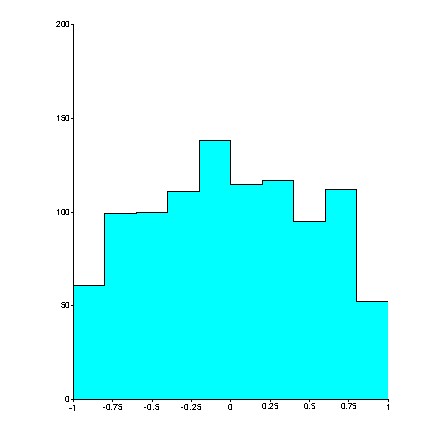
\includegraphics{histogram_corr.pdf}
\end{figure}

\begin{figure}
\center
\caption{Histogram of the squares of the correlation coefficients for 1000 sets of 5 random points.}
\label{histosquared}
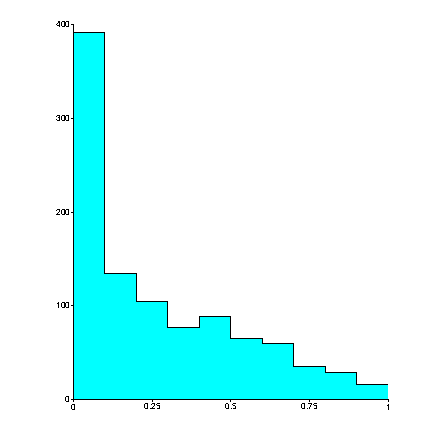
\includegraphics{histogram_squared.pdf}
\end{figure}

\section*{Effect of the number of data points}
If we consider data sets of different sizes, then it becomes clear that the very large correlation coefficients
that abound for very small sets, rapidly become rare when the set size increases (see Figure \ref{effectsize}).
If the set size is 5, then the absolute value of the correlation coefficient is between 0.9 and 1.0 for only
4\% of the time. On the other hand, the probability of a value between 0.5 and 0.7 is still more than 15\%.

But it is also clear that absolute values in the range 0.2 to 0.5 are very common even with a data set of
20~random points. The green line in the figure shows no clear decay. Extending the experiment to 100~data points
shows that it takes at least 70~points to get the probability of an absolute correlation coefficient between 0.2 and~0.5
down to 10\% (see Table \ref{table100}).

Clearly, one has to be careful putting too much value in the correlation coefficients found with even moderate size
data sets.

\begin{table}[h!]
\center
\caption{Number of correlation coefficients in a given range out of a set of 1000.}
\label{table100}
\begin{tabular}{lll}
\hline
\emph{Number of data points} & \emph{0.2 -- 0.5} & \emph{$>$ 0.5} \\
\hline
          20                 &           408     &     26        \\
          30                 &           311     &      7        \\
          40                 &           212     &      0        \\
          50                 &           156     &      0        \\
          60                 &           136     &      0        \\
          70                 &           102     &      0        \\
          80                 &           84      &      0        \\
          90                 &           61      &      0        \\
          100                &           51      &      0        \\
\hline
\end{tabular}
\end{table}

\begin{figure}
\center
\caption{Range of correlation coefficients (absolute values) as a function of the number of random points.
The y-axis shows the number of occurrences out of a total of 1000.}
\label{effectsize}
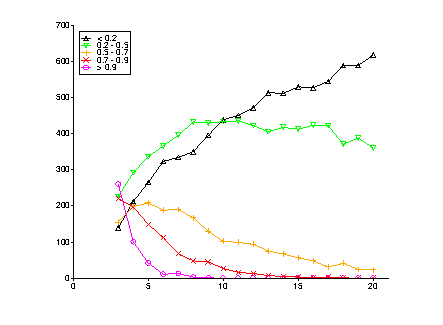
\includegraphics{effect_set_size.pdf}
\end{figure}

\end{document}
